\documentclass[11pt]{article}
\usepackage{listings}
\usepackage{amsfonts}
\usepackage{graphicx}
\newcommand{\numpy}{{\tt numpy}}    % tt font for numpy

\topmargin -.5in
\textheight 9in
\oddsidemargin -.25in
\evensidemargin -.25in
\textwidth 7in

\begin{document}

% ========== Edit your name here
\author{Francesco Penasa}
\title{Homework-6}
\maketitle

\medskip

% ========== Begin answering questions here
\begin{enumerate}

\item
\textbf{Exploit Buffer Overflow vulnerability to login using an arbitrary password.}

In order to login using an arbitrary password we overwrite the variable \textit{secret} using the buffer overflow vulnerability.
We write on the variable \textit{password} 20 characters, the first ten characterd will actually be stored in the password variable and the other ten will be stored in the previous variable in the code. For instance if we answer to the question \\ 
\textit{Please enter the password:} with \textbf{password12password34} \\
the variables used in the program will be
\begin{lstlisting}[language=C]
 char secret[10] = "password34";
 // char version[3] = "1.0";
 char password[10] = "password12";
\end{lstlisting}
Thanks to this vulnerability we are able to overwrite the variable \textit{secret} with an arbitrary string and make the condition \textit{(strncmp(password, secret, 10) == 0)} true. \\
In the case where other variables are declared in between \textit{password} and \textit{secret} we can still exploit this vulnerability by inserting some more random characters to overwrite the middle variables.
For instance if we answer to the question \\ 
\textit{Please enter the password:} with \textbf{password12nulpassword12} \\
the variables used for the login will be
\begin{lstlisting}[language=C]
 char secret[10] = "password12";
 char version[3] = "nul";
 char password[10] = "password12";
\end{lstlisting}
and we will be able to exploit the vulnerability successfully.

\item
\textbf{Fix Buffer Overflow vulnerability.} \\
To fix such vulnerability we could do a check on the length of the input string, to enable such check we can use the function \textit{fgets(...)} that limit the number of characters that can be specified in input instead of the function \textit{gets(...)} that does not perform such check. \\
So we simply substitute the function call \textit{gets(password);} with  \textit{fgets(password, 10, stdin);}\\

In the next page the screeshot of the mitigated C code is displayed.

\begin{figure}
\centering
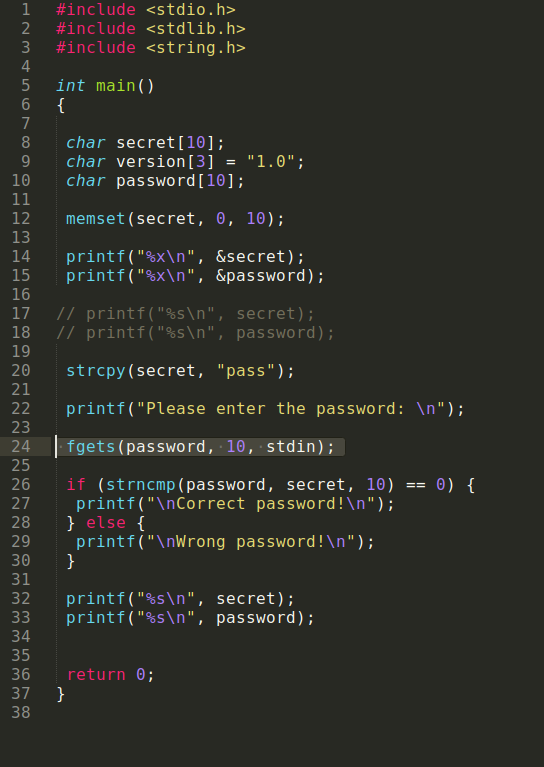
\includegraphics[scale=0.65]{image.png}
\end{figure}

\end{enumerate}
\end{document}
\grid
\grid